\paragraph{} Esta es la página para modificar elementos en la base de datos de una manera sencilla. Aquí se muestra al administrador un formulario con un campo por característica del microcontrolador, con la información actual sobre el mismo ya cargada, y que el administrador puede modificar a su gusto. El campo \textbf{''Referencia''} no será editable.

\paragraph{} Al pulsar el botón situado a la derecha se modifica el elemento en la base de datos y automáticamente se redirigirá al administrador a la página de listado completo, con el nuevo microcontrolador ya incluido en la lista.

\begin{figure}[h!]
	\centering
	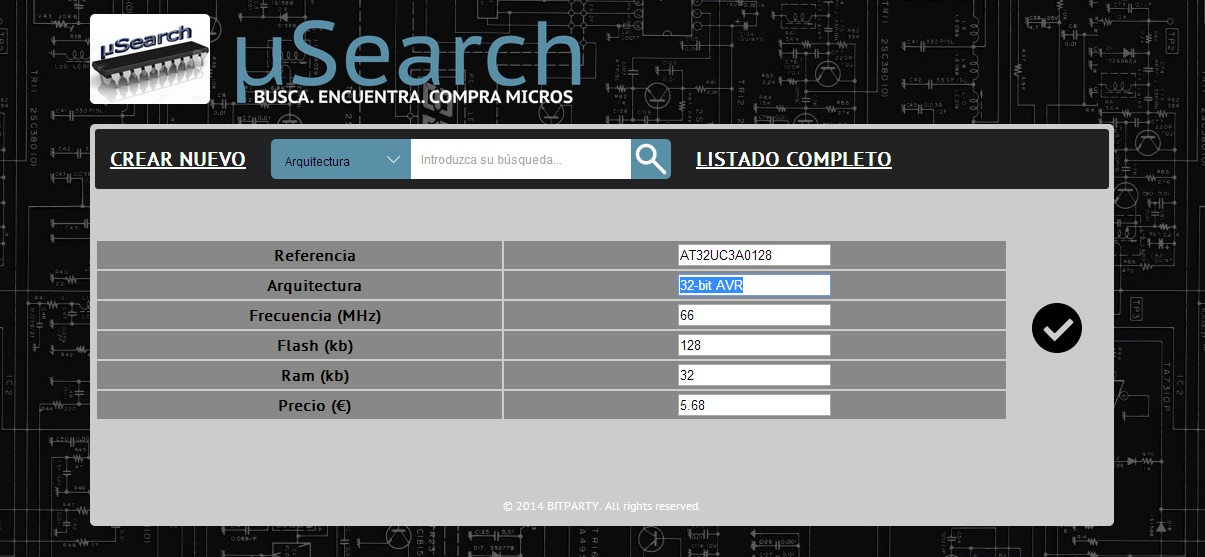
\includegraphics[width=0.75\textwidth]{img/editar}
	\caption{Página para modificar un micro-controlador.}
	\label{fig:editar}
\end{figure}

\paragraph{}Además, desde esta página de edición, a través de los iconos situados en la cabecera debajo de los logotipos de la web, el administrador puede acceder a:

\begin{itemize}
	\item \textbf{Crear Nuevo:} Redirige al administrador a la página para añadir un nuevo microcontrolador al catálogo electrónico.

	\item \textbf{Búsqueda:} Desde esta sección, el administrador puede realizar búsquedas sobre el catálogo de microcontroladores en base a cualquiera de sus características (Arquitectura, Frecuencia, Flash, RAM). Se debe seleccionar una de las características de la lista despegable, introducir el texto a buscar y pulsar sobre el icono de búsqueda.
	El administrador será redirigido a una página donde se le mostrará el resultado de la búsqueda.
			
	\item \textbf{Listado Completo:} Redirige al administrador a la página en la que se listan todos los microcontroladores disponibles en el catálogo.
\end{itemize}